
\section{多道程序系统与分时操作系统}

\subsection{多道程序系统}

现代的计算机已经不仅仅作为数字计算的工具,进入大众生活的计算机被赋予了更多生活上的需求,
用户可能在看电影的同时查看电子邮件,也有可能在写论文的时候进入浏览器查询相关资料,
但是更重要的是计算机往往在用户不经意间打开防病毒软件等保证用户计算机的安全。

由此可见多进程的工作方式在计算机工作中不可缺少。

但是在实际的处理过程中,计算机并不能同时处理多个程序。

首先要处理的问题是如何运行多个程序,早期的多道程序设计的出发点是充分的利用CPU,
作为输入设备的打孔纸带与CPU速度相比差距过大,昂贵的CPU常常在等待I/O信号而闲置。

具体情形如:A作业等待磁盘或者其他I/O时,CPU暂停为A作业服务,而转向为已完成I/O操作的B作业服务,
等到B需要执行下一步I/O操作时,CPU发现A作业完成了I/O操作,又转向为A作业服务,依次循环直到队列中所有作业完成。

由于A作业和B作业并行存储在计算机内存中,虽然在具体的执行中多次交换先后顺序执行,
但两个作业输出在同一个磁盘,故认为是多道程序在计算机中运行。

\subsection{分时操作系统}

分时是使得在用户看来计算机的多道程序同时运行,但是同时运行这也是不可能的。

所以只能采取折中的办法,使得CPU在用户不能明显感觉到的时间间隔内切换运行多个程序,
在切换后每个程序都能对作业进行一定的处理,在进行多个周期后,各个程序先后完成作业。

“不能明显感觉到的时间间隔内切换”中有两个概念,时间间隔和切换:

\begin{enumerate}
\item 时间间隔太长则用户会有明显的卡顿感,不利于分时概念的实现,
  而时间间隔太短则时间不足以让程序响应并完成一定量的工作,同样不利于分时概念的实现。
\item 切换涉及到保存当前程序的运行状态以便于程序获得CPU时间后可以接续上次的任务继续执行。
\end{enumerate}

\subsection{定时器}

定时器的实现是实现分时操作系统的关键,定时器每隔一段时间就向CPU发送中断信号,并记录发送的次数,以定时器发送的中断次数作为定时的依据。

管理定时器主要是使用PIT\footnote{PIT连接IRQ0,设定PIT就可以设定IRQ0的中断间隔,中断频率=单位时间事钟周期书(主频)/设定的数值}
(Programmable Interval Timer),之前说到定时器时间太短不利于分时的实现,故暂定1秒中发生100次中断。

在实际的运用中,往往需要用到不止一个定时器,于是需要对多个定时器进行管理,数据结构如图~\ref{lst:multi_timer}所示。

\begin{listing}[H]
  \inputminted[tabsize=2, firstline=175, lastline=187,
    linenos=true]{c}{../ZOS/src/kernel/bootpack.h}
  \caption{数据结构-多定时器}
  \label{lst:multi_timer}
\end{listing}

\begin{description}
\item[Timer *next:]下一个定时器地址;
\item[timeout:]下一个超时时刻;
\item[flags, flags2:]各个定时器的状态,在应用程序结束时定时器是否取消的标记
\item[count, next:]当前时刻,下一个时刻;
\item[Timer *t0:]所有时刻都要减去这个值。
\end{description}

对每个定时任务设置到超时时刻(对每个任务的运行时间进行计量,超过指定时刻向系统发送指令),
这样可以对一些设定了定时的任务在时间到了之后执行指定操作,
如光标的闪烁,页面的刷新等。

\subsection{任务切换}

在多道程序系统和分时操作系统分时操作系统完成后,任务切换就可以进行了。

任务切换从字面上理解很简单,多个任务之间来回切换,但是任务切换在计算机中实现却不那么简单。

如现有A和B两个任务,A正在运行,现在需要切换到B。
\begin{enumerate}
\item 任务B向CPU发送切换任务的指令
\item CPU把当前寄存器中的值全部写到内存中
\item CPU执行任务B
\item CPU切换到任务A并把所有寄存器中的值从内存中读出来,继续执行任务A
\end{enumerate}
流程如图~\ref{fig:tasksw}所示。
\begin{figure}[H]
  \centering
  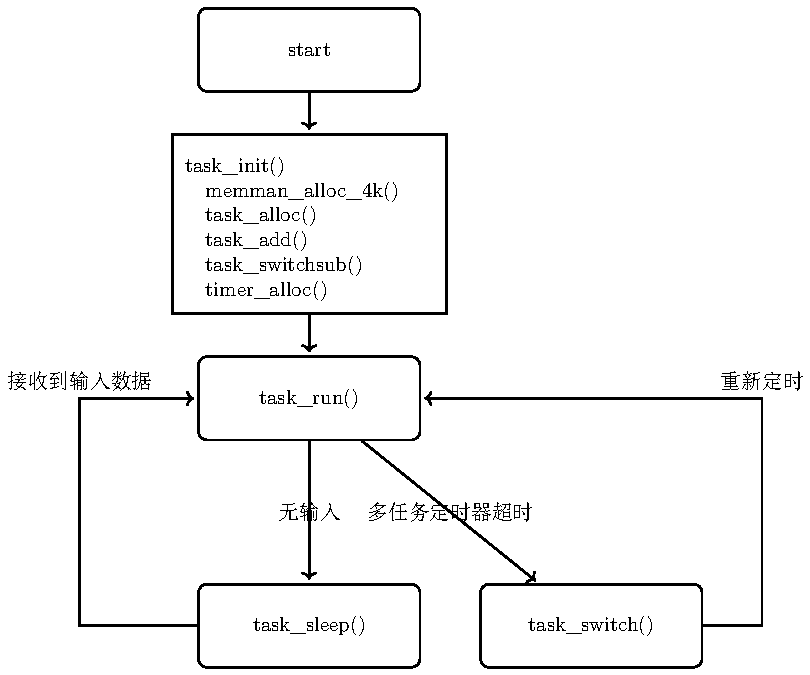
\includegraphics[width=.7\textwidth]{../Fig/func/multi.pdf}
  \caption{任务切换}
  \label{fig:tasksw}
\end{figure}

为了实现复杂的任务管理,需要用到的数据结构代码参见程序~\ref{lst:multi_task}。
\begin{listing}[H]
  \inputminted[tabsize=2, firstline=227, lastline=232,
    linenos=true]{c}{../ZOS/src/kernel/bootpack.h}
  \inputminted[tabsize=2, firstline=222, lastline=226,
    linenos=true]{c}{../ZOS/src/kernel/bootpack.h}
  \inputminted[tabsize=2, firstline=209, lastline=221,
    linenos=true]{c}{../ZOS/src/kernel/bootpack.h}
  \caption{数据结构-多任务}
  \label{lst:multi_task}
\end{listing}

\subsection{任务优先级}

在实际的运用中,所有任务在同一个优先级的安排显然是不合理的,
比如系统在执行A作业时,由于A作业和键盘输入作业优先级相同,
所以系统可能认为应该先完成A作业再执行键盘输入。

而通常人为操作中键盘优先级应该是最高的,为此设计任务的优先级。

\begin{listing}[H]
  \inputminted[tabsize=2, firstline=222, lastline=226,
    linenos=true]{c}{../ZOS/src/kernel/bootpack.h}
  \caption{数据结构-任务优先级}
  \label{lst:task_level}
\end{listing}

设计将任务分为多个层次,将音乐、网络传输等对优先级要求高的任务放在最高的优先级,
将鼠标等任务放在稍低的优先级,将对优先级要求低的任务放在较低的优先级,代码参见附录程序~\ref{lst:task_level}。

则系统在多任务同时运行的情况下会优先处理高优先级的任务,处理完成后处理稍低的优先级任务,
优先级较低的任务将在系统较空闲(即无更高优先级任务)的时候处理。